\documentclass[conference]{IEEEtran}
\usepackage{times}

% numbers option provides compact numerical references in the text. 
\usepackage[numbers]{natbib}
\usepackage{multicol}
\usepackage{amsmath}
\usepackage{graphicx}
\usepackage{float}
\usepackage[bookmarks=true]{hyperref}

\pdfinfo{
   /Author (Homer Simpson)
   /Title  (Robots: Our new overlords)
   /CreationDate (D:20101201120000)
   /Subject (Robots)
   /Keywords (Robots;Overlords)
}

\usepackage{CJKutf8}

\begin{document}
\begin{CJK}{UTF8}{gbsn}

% paper title
\title{ Adaptive Quadruped Robot Parkour via Task-targeted Curriculum and Heading-aware Distillation}

% You will get a Paper-ID when submitting a pdf file to the conference system
\author{陆紫萌 524531910001    
裘嘉敏 524030910068    
范文茜 524531910002}

%\author{\authorblockN{Michael Shell}
%\authorblockA{School of Electrical and\\Computer Engineering\\
%Georgia Institute of Technology\\
%Atlanta, Georgia 30332--0250\\
%Email: mshell@ece.gatech.edu}
%\and
%\authorblockN{Homer Simpson}
%\authorblockA{Twentieth Century Fox\\
%Springfield, USA\\
%Email: homer@thesimpsons.com}
%\and
%\authorblockN{James Kirk\\ and Montgomery Scott}
%\authorblockA{Starfleet Academy\\
%San Francisco, California 96678-2391\\
%Telephone: (800) 555--1212\\
%Fax: (888) 555--1212}}


% avoiding spaces at the end of the author lines is not a problem with
% conference papers because we don't use \thanks or \IEEEmembership


% for over three affiliations, or if they all won't fit within the width
% of the page, use this alternative format:
% 
%\author{\authorblockN{Michael Shell\authorrefmark{1},
%Homer Simpson\authorrefmark{2},
%James Kirk\authorrefmark{3}, 
%Montgomery Scott\authorrefmark{3} and
%Eldon Tyrell\authorrefmark{4}}
%\authorblockA{\authorrefmark{1}School of Electrical and Computer Engineering\\
%Georgia Institute of Technology,
%Atlanta, Georgia 30332--0250\\ Email: mshell@ece.gatech.edu}
%\authorblockA{\authorrefmark{2}Twentieth Century Fox, Springfield, USA\\
%Email: homer@thesimpsons.com}
%\authorblockA{\authorrefmark{3}Starfleet Academy, San Francisco, California 96678-2391\\
%Telephone: (800) 555--1212, Fax: (888) 555--1212}
%\authorblockA{\authorrefmark{4}Tyrell Inc., 123 Replicant Street, Los Angeles, California 90210--4321}}


\maketitle

\begin{abstract}
  We propose to develop a quadruped robot capable of executing extreme parkour tasks in simulation, leveraging vision-based reinforcement learning. Our approach builds upon the Extreme Parkour baseline and enhances it through two main components. The first is task-targeted curriculum learning to independently scale difficulty by obstacle type, which improves learning efficiency and policy generalization. The second is pretrained heading prediction and teacher-to-student distillation, explicitly separating “where to go” from “how to move” to improve directional precision on narrow or misaligned obstacles.

\setlength{\parindent}{2em}  We expect our robot to perform jumps, gaps, and step sequences with high success rates on both standard and novel terrains, including challenging bean gaps, biased gaps, and randomized \textit{parkour v2 }courses.
\end{abstract}

\IEEEpeerreviewmaketitle

\section{Motivation and Problem Statement}

Inspired by \citet{cheng2024extreme}, we identify two limitations in existing learning-based parkour methods. First, curriculum learning is often applied globally, which may overemphasize easier tasks while insufficiently exploring more difficult obstacles. Second, student policies typically lack explicit heading pretraining, which can reduce stability on direction-sensitive terrains. To address these issues, we propose a task-targeted curriculum that adjusts difficulty separately for each obstacle type, together with a heading-aware distillation framework that pretrains heading prediction before action distillation. Our goal is to learn a policy that maps depth images and proprioceptive inputs to joint actions, enabling safer and more robust traversal of parkour terrains such as hurdles, gaps, alternating steps, and ramps.


\section{Literature Review}
Recent learning-based legged locomotion methods directly map sensory observations to motor actions and have shown strong agility on complex terrains \cite{2021arXiv210704034K, Tsounis2019DeepGaitPA}. Extreme Parkour further shows that a two-phase teacher-student framework can learn highly dynamic parkour behaviors from depth images \cite{cheng2024extreme}. Yet two limitations remain relevant to parkour learning: globally applied curriculum learning may overlook obstacle-specific difficulty and hinder efficient training on harder terrains \cite{Smith-RSS-23}, while implicitly learned directional intent can reduce stability on heading-sensitive obstacles \cite{Margolis2021LearningTJ}. These observations motivate task-targeted curriculum design and more explicit heading-aware policy learning.



\section{Technical Plan}

\subsection{New Obstacle and Terrain}

To further enhance the parkour capability of quadruped robots across more diverse terrains, we designed four new obstacle types and terrains: beam gap, staggered gap, slanted hurdle, and parkour v2 (Figure \ref{fig:terrains}).

\begin{figure}[h]
    \centering
    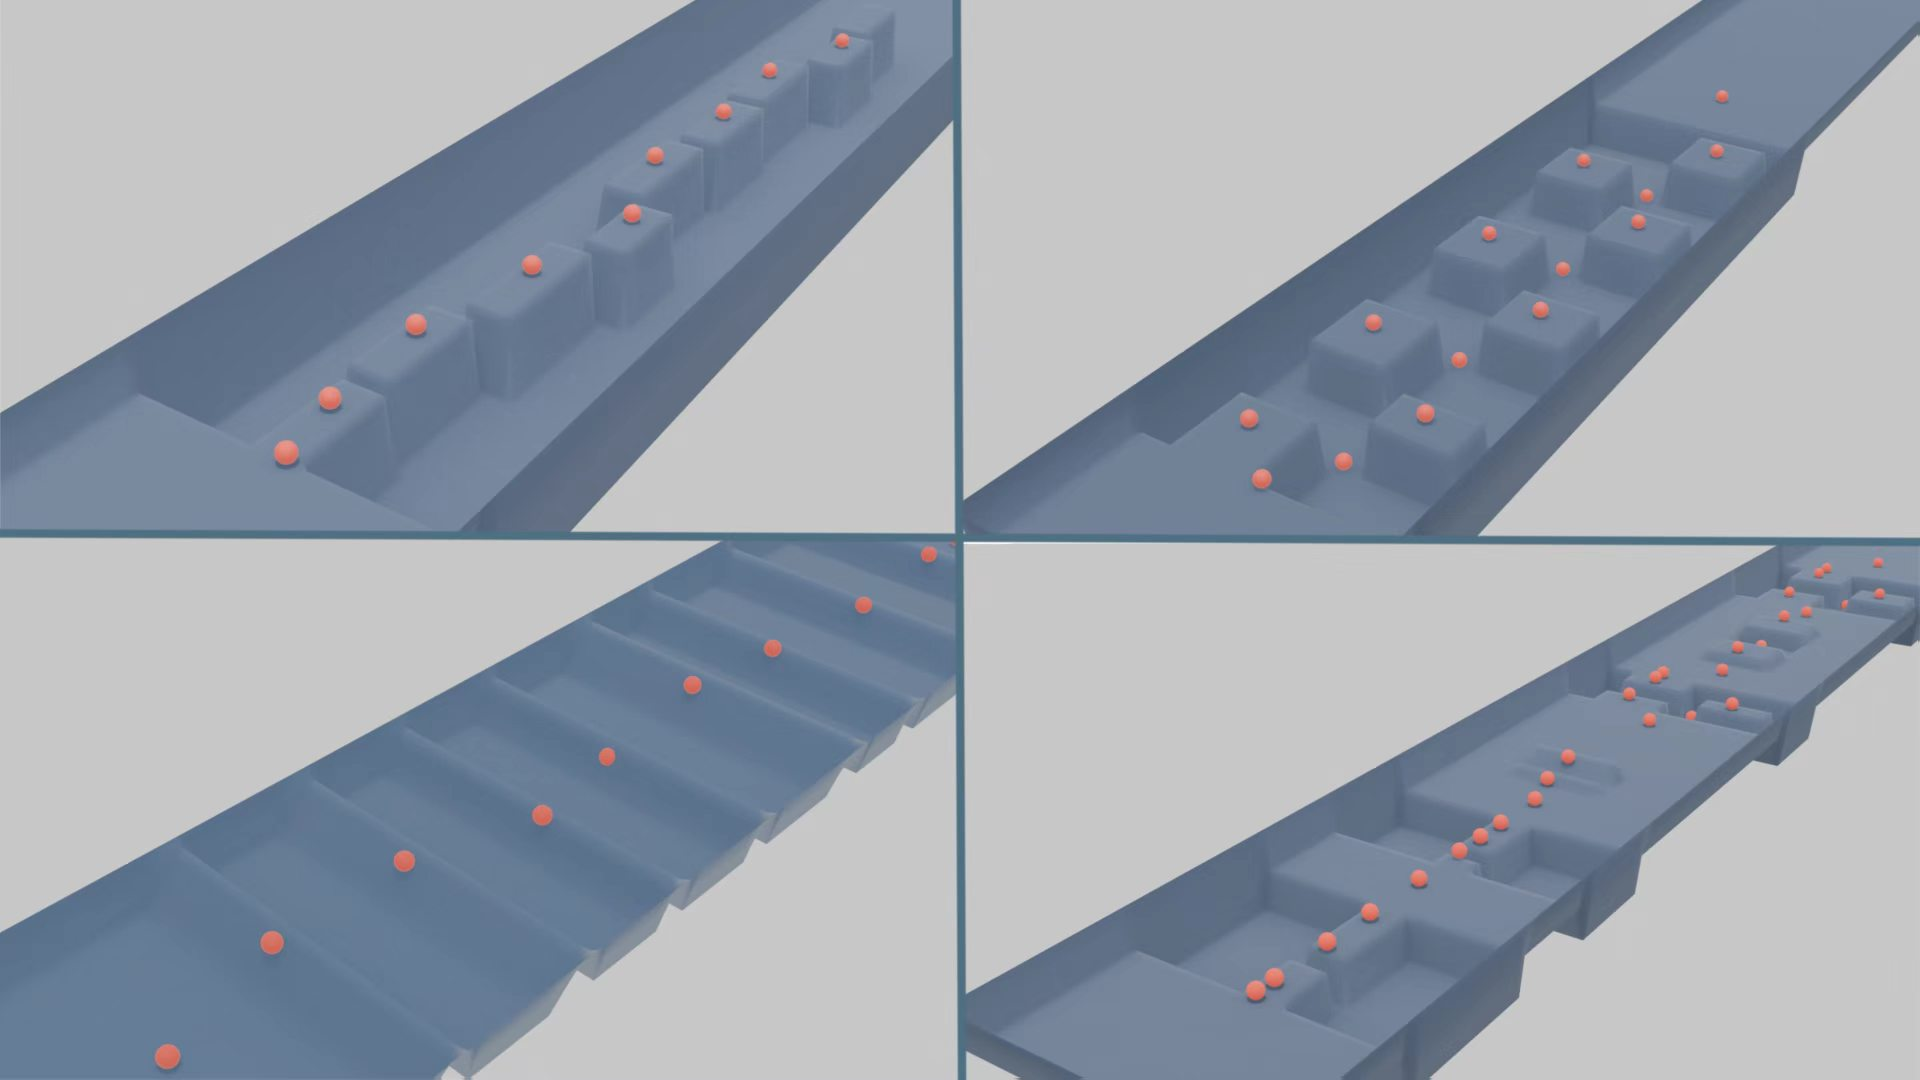
\includegraphics[width=\linewidth]{figures/terrains.jpg}
    \caption{The four newly designed terrains (top-left to bottom-right): Beam gap (tests lateral deviation and $r_{clearance}$); Staggered gap (evaluates heading accuracy and foothold planning); Slanted hurdle (assesses adaptation to continuous obstacles); Parkour V2 (mixed terrains to verify strategy generalizability).}
    \label{fig:terrains}
\end{figure}


\subsection{Pretrained Heading Predictor}

We make the \textbf{heading prediction} stage explicit. Instead of treating heading as an internal part of student distillation, we introduce a dedicated module that predicts a body-frame heading vector from proprioception and depth, and then feeds this feature into the action policy. The student model contains a shared visual backbone, a heading head, and a terrain latent head, while the actor takes proprioception, predicted heading, and depth latent as input (Figure~\ref{fig:stu-model}). This design decouples ``where to go'' from ``how to move,'' which is especially useful for direction-sensitive obstacles such as bean gap and staggered gap.

\begin{figure}
    \centering
    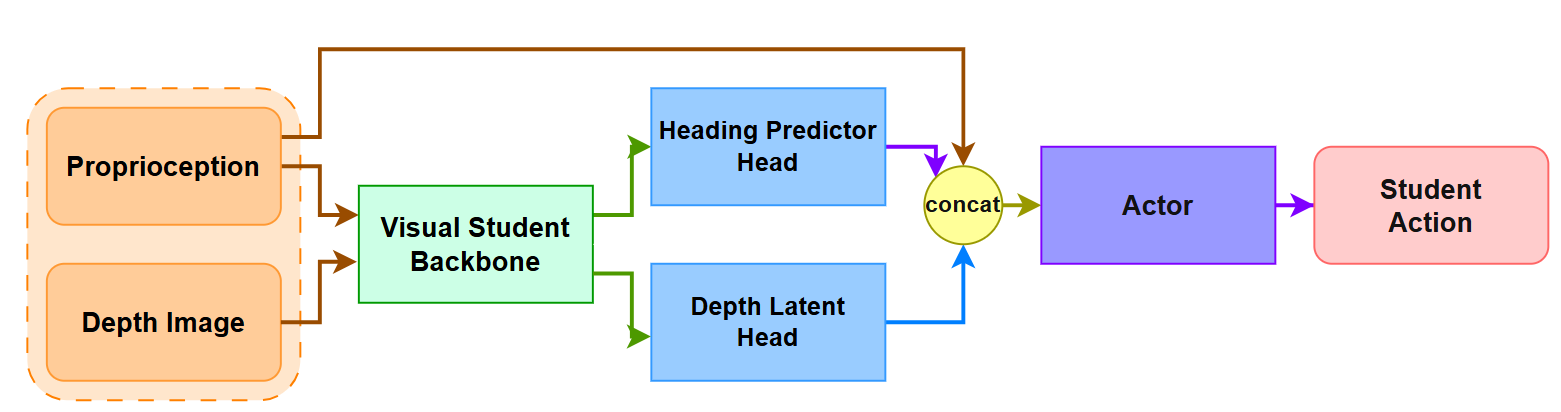
\includegraphics[width=\linewidth]{figures/stu-model.png}
    \caption{Student model with explicit heading prediction. A shared backbone extracts visual features, followed by heading and terrain-latent heads. The predicted heading and latent are fused with proprioception and fed to the actor.}
    \label{fig:stu-model}
\end{figure}

Training has three stages: (1) pretraining the backbone and heading head with teacher-generated body-frame heading labels while freezing the actor; (2) distilling teacher actions using predicted heading and terrain latent; and (3) optional end-to-end fine-tuning with a joint loss:
\begin{align}
L_{\text{heading}} &= \frac{1}{T} \sum_{t=1}^{T} \| \hat{\mathbf{h}}_t - \mathbf{h}^{\text{teacher}}_t \|_2^2 \\
L_{\text{action}} &= \frac{1}{T} \sum_{t=1}^{T} \| \mathbf{a}_t^{\text{student}} - \mathbf{a}_t^{\text{teacher}} \|_2^2 \\
L_{\text{latent}} &= \frac{1}{T} \sum_{t=1}^{T} \| \mathbf{z}_t^{\text{student}} - \mathbf{z}_t^{\text{teacher}} \|_2^2 \\
L_{\text{total}} &= w_h L_{\text{heading}} + w_a L_{\text{action}} + w_l L_{\text{latent}}
\end{align}
This progressive design preserves the reproduced baseline actor while testing whether explicit heading supervision improves control.

\subsection{Task-Targeted Curriculum}

We extend the original global terrain curriculum into a \textbf{task-targeted curriculum}. Instead of using immediate per-environment performance, we maintain separate curriculum states for different terrain types and update them with \textbf{fixed-window statistics}. Each task thus progresses at its own pace, with hysteresis thresholds to reduce oscillation. Since hurdle, gap, step, and ramp-like terrains differ substantially in geometry and difficulty, this design is intended to improve training stability, balance task coverage, and avoid under-training harder tasks.

\subsection{Reproduction Progress}

So far, our work has established a verified baseline training pipeline for extreme-parkour on remote GPU servers. We successfully launched base-policy training, ran it to 50 iterations, and confirmed checkpoint saving works correctly.

\section{Expected Outcome}
\setlength{\parindent}{2em}
We expect the proposed framework to enable robust quadruped parkour across both standard and newly designed terrains. Specifically, we anticipate:

\begin{itemize}
\item Better generalization to unseen terrains;
\item Higher success rates and mean x-displacement (MXD) on challenging obstacles;
\item Improved directional accuracy and more stable locomotion;
\item Faster and more balanced learning across tasks.
\end{itemize}

Overall, these results are expected to show that heading-aware distillation and task-specific curriculum learning improve the performance and robustness of learned parkour policies.

\section{Potential Risks and Backup Plan}
\setlength{\parindent}{2em}

The potential risks and corresponding backup plans for our project are as follows:

\begin{itemize}
    \item The model may have limited generalization on highly challenging terrains we designed. As a backup plan, we can relax the conditions for certain terrains.
    \item The addition of the heading predictor may lead to slower inference speed and increased action latency. As a backup plan, we can reduce the number of model parameters or optimize the inference pipeline.
    \item The low success rate on more demanding tasks may slow down the overall training progress. As a backup plan, we can merge fine-grained tasks into a few coarser categories or adopt larger sliding windows for statistics.
    \item Limited computational power may lead to slower-than-expected training progress. As a backup plan, we can optimize the training pipeline or reduce the parameter count.
    \item Segmentation faults still occur in distillation and inference workflows, even though the Ubuntu, Isaac Gym, and PyTorch versions appear compatible. As a backup plan, we can decouple training and playback. 
    %continue training on the remote server to reliably produce checkpoints, then transfer checkpoints to a local Ubuntu machine and run play.py locally for rollout verification and visualization.
\end{itemize}

%As backup plans, we provide serveral solutions:




%The proposed framework faces several risks, including limited generalization on highly challenging terrains, unstable heading prediction on narrow or offset gaps, unreliable curriculum updates under sparse obstacle samples, and an unresolved segmentation fault in both distillation runs and \texttt{play\_headless\_record.py}.


%For the segmentation fault, we will prioritize numerical evaluation without recording, isolate the crash with a minimal reproducible script, and, if unresolved, focus on the curriculum component while treating heading-aware distillation as an extension.


\section{Timeline}

\setlength{\parindent}{2em}
\begin{table}[H]
\centering
\caption{Project Timeline and Milestones}
\begin{tabular}{|c|p{7cm}|}
\hline
\textbf{Week} & \textbf{Milestone / Task} \\
\hline
8 & Implement the baseline quadruped parkour policy in Isaac Gym; reproduce standard terrains and validate basic locomotion. \\
\hline
9-10 & Design and implement new obstacle types: alternating steps, beam gaps, biased gaps, and \textit{parkour v2} courses; apply task-targeted curriculum to improve convergence. \\
\hline
11-12 & Pretrain the heading predictor; verify heading predictions on complex terrains; freeze the backbone if needed.  \\
\hline
13 & Distill student policy with predicted heading and depth latent. \\
\hline
14-15 & Conduct ablation studies and full-policy evaluation on standard and newly designed terrains; collect metrics including success rate and heading accuracy; categorize typical failure cases; prepare final report and demo. \\
\hline
\end{tabular}
\end{table}
\section*{Acknowledgments}

%% Use plainnat to work nicely with natbib. 

\bibliographystyle{unsrtnat}
\bibliography{references}

\end{CJK}
\end{document}
